\section{Descripción del Software y Manual de Uso}

\subsection{Forma de importar los datos al sistema}
La informacion desde los archivos de texto codificados en ascii se importan por
medio de un script en python. El script toma cada archivo y genera una carpeta
con un nombre y además con el sufijo FOLDER. Consideremos como ejemplo el
archivo de sismograma con el nombre
\subsection{Descripción de estructuras de datos}
Las información de un evento está almacenada en dos clases matlab con los
nombres event.m y geonsensor.m los cuales están relacionados como se muestra en
la figura. 

\subsection{Resumen de implementacion (En Matlab y Python)}

\subsubsection{Scripts en Python}
\paragraph{readFile.py}
Se usa una rutina en python para separar la información desde los documentos de
los geofonos y convertirla a archivos que servirán de imput que funciones matlab
trasnformen la información a objetos matlab.
\paragraph{patterns.py}
Conjunto de patrones con la información necesaria que luego se extraerá mediante
readFile.py.

\subsubsection{Clases Matlab}
\paragraph{Event.m}
Clase que contiene una lista de geosensores y los parámetros de un evento
sísmico específico. Estos son los atributos de los set de datos entregados
por Codelco.
\paragraph{Geonsensor.m}
Clase que contiene la información de cada uno de los geofonos en un evento
específico. 
\subsubsection{Documentación de las Rutinas Principales}

\paragraph{Importar información a matlab}
\begin{itemize}
  \item Archivo: script/importEvents.m
  \item Comando: events = importEvents()
  \item Descripción: Almacena la información desde los archivos tratados por el
  script python readFile.py a una vector de objetos Event en matlab.
  \item input: no recibe parámetros de entrada dado que hace lecturas sobre
  archivos de texto almacenados en disco.
  \item output: event lista de objetos del tipo Event que contienen a todos los
  eventos sísmicos almacenados en la carpeta `./project/data sets`  		 
\end{itemize}


\paragraph{Estimar la fuente sismica de un evento sísmico}
\begin{itemize}
  \item Archivo: script/source.m
  \item Comando: [src, filtsrc, error] = source(event, nSrc, L, por)
  \item Descripción: Estima la fuente como una fuerza $f(t)$ en un intervalo de 
  tiempo de largo $L$ dado el conjunto de sismógrafos del evento
  \textbf{event} con una discretización del dominio con \textbf{nSrc} con una
  fracción \textbf{por} de la fuente antes de \textbf{event.origin\_time} es
  cual es el valor estimado por codelco.
  \item input: 
    \begin{itemize}
    \item event: Objeto del tipo Event el cual representa el sísmico del cual se
    quiere obtener la estimación de la fuente $f(t)$ como una fuerza.
    \item nSrc: número de puntos de la discretización uniforme en el tiempo con
    la cual se va a estimar la fuente.
    \item L: largo de la ventana de tiempo en donde se va a estimar la fuente
    \item por: porcentaje de la ventana de tiempo que está antes del tiempo de
    origen estimado por el documento del evento.
    \end{itemize}
  \item output:
  	\begin{itemize}
  	  \item src: fuente sismica como una fuerza en el punto $r_0$ estimado desde
  	  los valores dados por las mediciones de los geofonos
  	  \item filtsrc: src pero filtrada eliminando los modos bajos
  	  \item error: error de estimación 
  	\end{itemize}
\end{itemize}

\paragraph{script/constructsensor.m}

Deduce la forma de un geofono dada una fuente sísmica
\subsection{Manual de uso}
El uso del programa está descrito en dos archivos matlab distintos, en el 
primero sampletimereversal.m se describe como invertir la señal en tiempo. En el
segundo archivo llamado sampleRecSource.m se describen los pasos para la 
reconstruccion de una fuente sismica a partir de la información de los geofonos 
dados por Codelco.


\begin{verbatim}
%lista de todos los eventos sismicos
events = importEvents()
%mostrar el primero y se vera que las variables de este objeto tienen el mismo
% nombre que las variables utilizadas en los set de datos
event(1)

>>
ans = 

  Event

  Properties:
              name: {'1998_aug_02_07_30_40.d5g'}
           beta_est: 3500
          alpha_est: 5600
          alpha_ind: []
           beta_ind: []
                gss: [1x8 Geosensor]
              alpha: 5600
               beta: 3500
                rho: 2700
         first_time: 40.5227
          last_time: 41.5579
              count: 8
               LocR: [-439.5702 -1.1564e+03 -2.1773e+03]
        origin_time: 40.5655
           tail_per: 0
              error: 0.1500
                 xi: -892.7790
                 xf: -20.2270
                 yi: -1.5404e+03
                 yf: -715.6420
                 zi: -2.2857e+03
                 zf: -1.9726e+03
                 dx: 14.7890
                 dy: 13.9790
                 dz: 34.7967
                 dt: []
                 nx: []
                 ny: []
                 nz: []
                 nt: []
            n_rsmpl: []
           max_norm: []
             x_axis: [1x60 double]
             y_axis: [1x60 double]
             z_axis: [1x10 double]
             t_axis: [1x50 double]
           X_domain: []
           Y_domain: []
           Z_domain: []
           T_domain: []
    origin_time_est: 40.5655
           LocR_est: [-439.5702 -1.1564e+03 -2.1773e+03]
                 r0: []
            all_est: []
     alpha_ind_post: []
      beta_ind_post: []
                src: []
            filtsrc: []
                  e: []
                 v1: []
                 v2: []
                 v3: []
                vr1: []
                vr2: []
                vr3: []
                  A: []
                  U: []
            indices: []
             alphas: []
\end{verbatim}


\subsubsection{Geonsensor.m} 
Clase que contiene los atributos de un geosensor especifico en un evento
sísmico. Contiene las mediciones y propiedades calculadas
necesarias para los algoritmos.
\paragraph{Ejemplo}
\begin{verbatim}
%lista de todos los eventos sismicos
events = importEvents()
%mostrar el primer geosensor de la lista de el evento 1
event(1).gss(1)
ans = 

  Geosensor

  Properties:
                   cuttime: 40.6138
                 firsttime: 40.5286
                  lasttime: 41.0173
       resampleErrorOnNorm: 0.1499
              resampleSize: 191
        timeresamplevector: [1x191 double]
                timevector: [1x4888 double]
        diferenciaPSvalida: 1
         medicionesValidas: [1 1 1]
                        r0: [-369.6930 -1.1323e+03 -2.1262e+03]
    hardware_sampling_rate: 10000
           resampling_rate: [1x190 double]
                    period: [1x190 double]
           TriggerPosition: 542
                  max_norm: []
                       r_x: [1x191 double]
                       r_y: [1x191 double]
                       r_z: [1x191 double]
                         L: 4888
                      data: [4888x3 double]
                    t_time: 40.5828
                    p_time: 40.5807
                    s_time: 40.5939
               rvrse_amplt: []
                    validP: 1
                    validS: 1
                   validSP: 0
           IsAccelerometer: 0
             IsSpeedometer: 1
                 sensor_id: 29
                  validAll: 1
\end{verbatim}

\subsection{Funciones principales}

\subsubsection{Source.m} 

Dado un evento s\'{\i}smico \textbf{event}, estima la fuente discretizado en \textbf{n}
puntos, con un ancho total de \textbf{width} segundos, comenzando la ventana temporal
de la fuente un tiempo \textbf{per}*\textbf{width} antes del tiempo de origen \textbf{origin\_time}.
\paragraph{Ejemplo}

\begin{verbatim}
%importamos los eventos sismicos
events = importEvents()
%seleccionamos uno de estos eventos, por ejemplo, el quinto
ev = events(5)
% estimacion de la fuente con 100 datos, con un ancho 0.3 y un 0.1 de la senal
% antes del tiempo de origen
 [src] = source(ev,100,0.3,0.1)
\end{verbatim}

\subsubsection{Reverse\_signal}
Realiza el time reversal ocupando como fuente las mediciones, invertidas en
el tiempo, de un evento específico.
\begin{verbatim}
%importamos los eventos sismicos
events = importEvents()
%seleccionamos uno de estos eventos, por ejemplo, el quinto e invertimos las
% sen~ales en el tiempo
[X,Y,Z] = events(5).reverse_signal;
% La visualizacion de la inversion
plotRevSignal(X,Y,Z);
\end{verbatim}

\subsection{Otras funciones}
\subsubsection{scalarGreenKernel.m}
\begin{verbatim}
function [G11,G12,G13,G22,G23,G33] = scalarGreenKernel(x,y,z,T, alpha, beta,rho)
\end{verbatim}
Retorna la función de Green para un vector de tiempo específico, para la
posici\'on $(x,y,z)$. Las velocidades de propagación de la onda son alpha y beta
y la densidad del medio es $\rho$.

Los pasos siguientes son para el uso del producto, es importante señalar que el
sistema fue desarrollador en matlab
\subsection{Importar desde los set de datos}

Para poder utilizar el producto se requiere tener un conjunto de archivos como 
los que entregan cada uno de los geosensores utilizados. Estos archivos,
mediante una rutina en python generan una carpeta para cada evento correspondiente con el 
nombre del evento como muestra en la figura.

\begin{verbatim}
>>~\ruta-rutina-python\ python readFiles.py
\end{verbatim}

\begin{figure}[H]
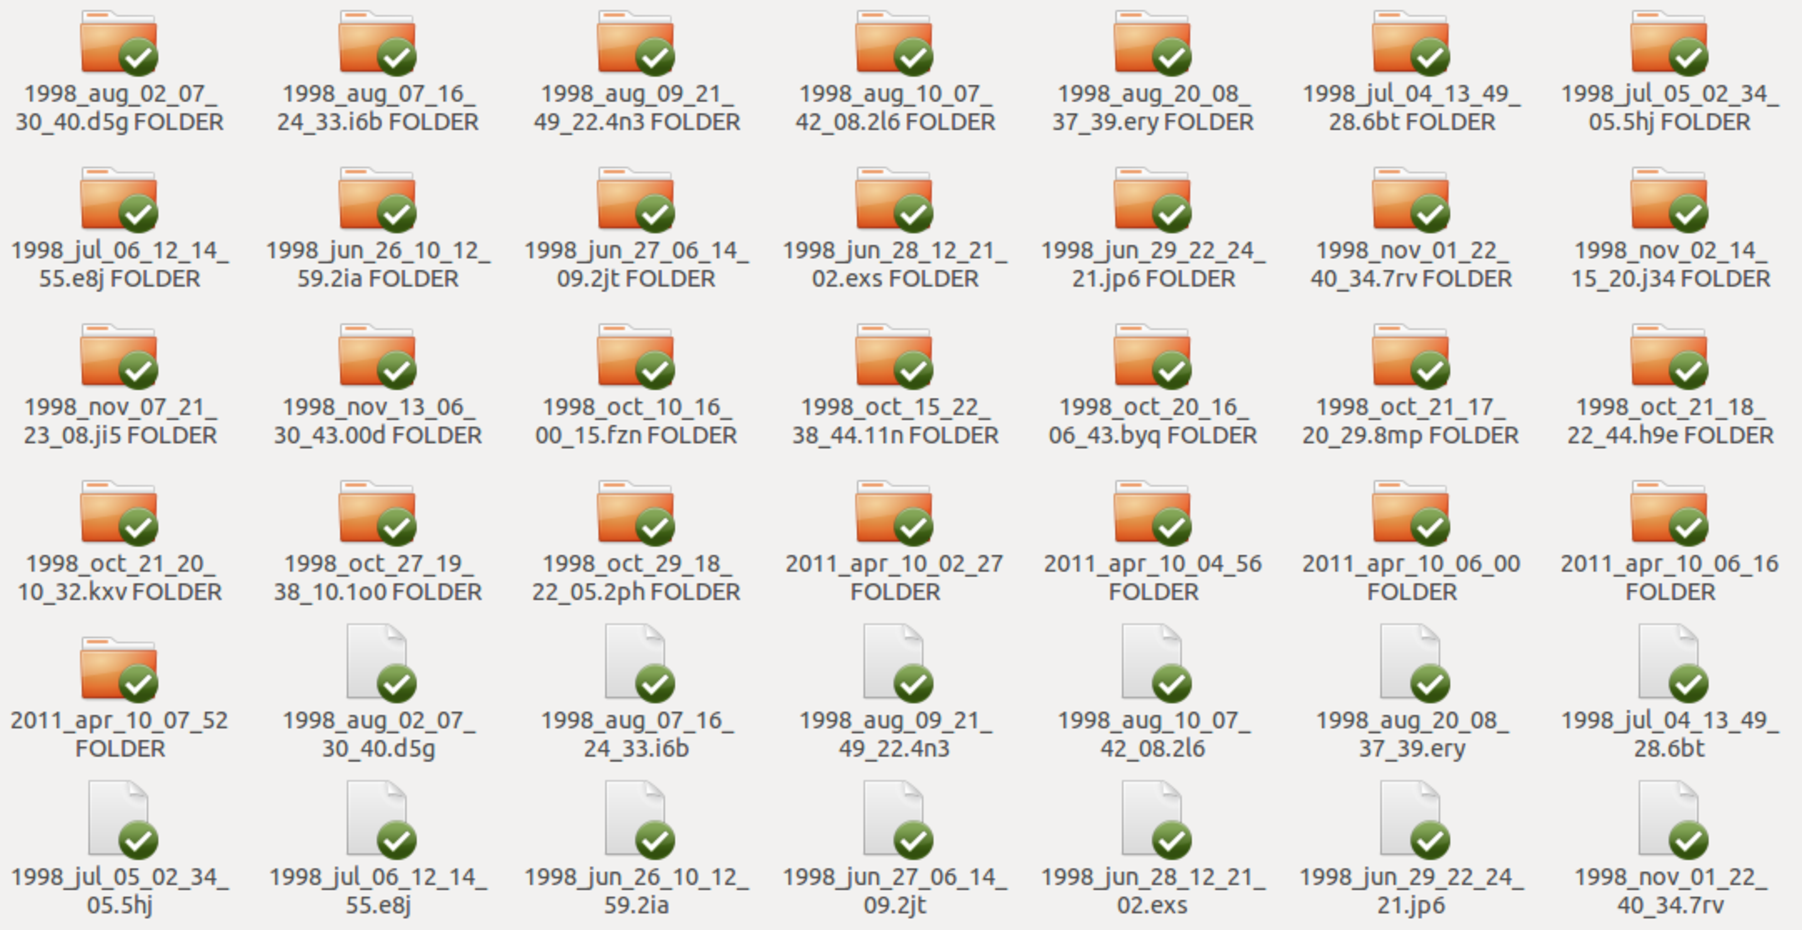
\includegraphics[width=0.9\textwidth,height=0.4\textheight]{linea_timerev/figuras/folders.pdf}
\caption{Archivos de codelco con su respectiva carpeta}
\end{figure}



Con lo cual todos los archivos se transformaran en carpetas con información que 
servirá de input para el programa en matlab.

\subsection{Importar información a los objetos matlab}
Estando en Matlab, con la carpeta matlab agregada en el path, podemos almacenar 
todos la información a objetos matlab.

\begin{verbatim}
events = ImportEvents();
\end{verbatim}
\subsection{Construcción de las fuentes para cada evento }
Para reconstruir la fuente de un evento seleccionado, se debe de elegir un evento
de el total
\begin{verbatim}
% se selecciona el evento 1 de la lista
event = events(1);
% se reconstruye la fuente, fuente filtrada y error bajo la norma 2
% nota: se ha identificado que existen sensores con mediciones malas, por
% ejemplo el sensor que tiene sensor_id = 25, se pueden eliminar los sensores a
% mano de tal manera de evitar resultador erroneos
event.gss(find([event.gss.sensor_id]==25)) = [];
event.count = length(event.gss);
tic;
% evento de 100 puntos
[src, filtsrc, err] = source(event,100, 0.5,0.09);
toc;
\end{verbatim}

\subsection{Rotar una señal filtrada para conocer el tipo de fuente}
Ya con una reconstrucción de la fuente s\'{\i}smica, se puede rotar la fuente
filtrada para ver como se proyecta la fuerza en cada uno de los ejes.
\begin{verbatim}
Ev.gss([Ev.gss.sensor_id] == 25) = [];
Ev(ii).count = length( Ev(ii).gss);
% eliminar sensor_id = 25

% se almacena informacion, como la fuente, fuente filtrada, error
[Ev.src, Ev.filtsrc, Ev.error, ~, Ev.U, ~, ~]= source(Ev,100, 0.5,0.09);  
% coeficientes de la fuerza proyectada en los ejes canonicos 
[Ev.v1, Ev.v2, Ev.v3] = EventCoeficients(Ev.src);
% coeficientes de la fuerza filtrada y rotada proyectada.
[Ev.vr1, Ev.vr2, Ev.vr3] = EventCoeficients(rotate(Ev.filtsrc));
% visualizacion de la fuente sismica rotada por componentes principales
plotSrc(rotate(Ev.filtsrc),Ev.origin_time);
\end{verbatim} 
